% =====================================================================
% CHAPTER 3 -- Summary of: M. K. T. Al-Nuaimi et al., IEEE AWPL, 2026 [AlNuaimi2026]
% =====================================================================
\section*{CHAPTER 3. OPTICALLY TRANSPARENT SES FOR 5G}
\addcontentsline{toc}{section}{\numberline{}CHAPTER 3. OPTICALLY TRANSPARENT SES FOR 5G}
\setcounter{section}{3}
\setcounter{subsection}{0}
\setcounter{equation}{0}
\setcounter{theorem}{0}
\setcounter{figure}{0}
\setcounter{table}{0}

\subsection{Problem}
The 5G mmWave bands n258 (24.25--27.5~GHz) and n257 (26.5--29.5~GHz) offer high data rates and low latency. They also suffer from high free-space path loss, limited diffraction and strong blockage, so buildings, walls and vegetation create coverage gaps in dense cities~\cite{AlNuaimi2026}. Electromagnetic skins (EMSs), also called intelligent reflecting surfaces, can redirect the BS signal into these gaps without consuming power. However, most EMSs are made of opaque dielectric and metal layers and look intrusive on fa\c{c}ades. Covering both n258 and n257 with a stable reflection angle is also difficult: the required phase profile changes with frequency, and the unit cells respond differently across the band~\cite{AlNuaimi2026}.

\subsection{Contributions and Methodology}
Al-Nuaimi \textit{et al.}~\cite{AlNuaimi2026} design, fabricate and measure an optically transparent, passive and wideband EMS that can be integrated into window glass (Fig.~\ref{fig:ch3-prototype}).
\begin{itemize}
    \item \textbf{Materials.} The conductor is a transparent indium-tin-oxide (ITO) film with a sheet resistance $R_{\mathrm{sheet}} = 2.5~\Omega$/sq (650~nm thick) on soda-lime glass. Two glass layers are separated by a 1~mm air gap, which widens the bandwidth, stabilizes the reflection phase and reduces losses.
    \item \textbf{Unit cell.} The cell is an octagonal ITO resonator. Two cell types (UC1 and UC2) are combined to cover the full $0^\circ$--$360^\circ$ phase range, with a period of $0.42\lambda$ at 26~GHz and $0.45\lambda$ at 28~GHz. CST simulations show that $R_{\mathrm{sheet}}$ changes only the reflection amplitude (loss), not the phase, and that the phase stays stable under oblique incidence.
    \item \textbf{Array design.} The EMS has $40 \times 40$ cells ($200 \times 200 \times 2.1$~mm). It is designed for a BS 10~m away, with incidence angle $\theta_i = 15^\circ$ and reflection angle $\theta_r = 37^\circ$. The phase of each cell is~\cite{AlNuaimi2026}
    \begin{equation}\label{eq:ch3-phase}
    \varphi(x_o,y_o) = -k_o \sin\theta_r \left(x_o\cos\phi_r + y_o\sin\phi_r\right) + k_o R_i ,
    \end{equation}
    where $(x_o, y_o)$ is the cell centre, $k_o$ the free-space wavenumber, $(\theta_r, \phi_r) = (37^\circ, 0^\circ)$ the reflection direction, and $R_i = 10$~m the BS--EMS distance. The first term of \eqref{eq:ch3-phase} tilts the reflected wavefront towards $\theta_r$; the second compensates the path from the BS.
    \item \textbf{Validation.} The prototype was made by laser etching. The team measured its optical transparency with a transmission meter, its reflection in an anechoic chamber with two horn antennas and a vector network analyzer (VNA), and the ITO sheet resistance with a four-point probe.
\end{itemize}

\begin{figure}[!htbp]
    \centering
    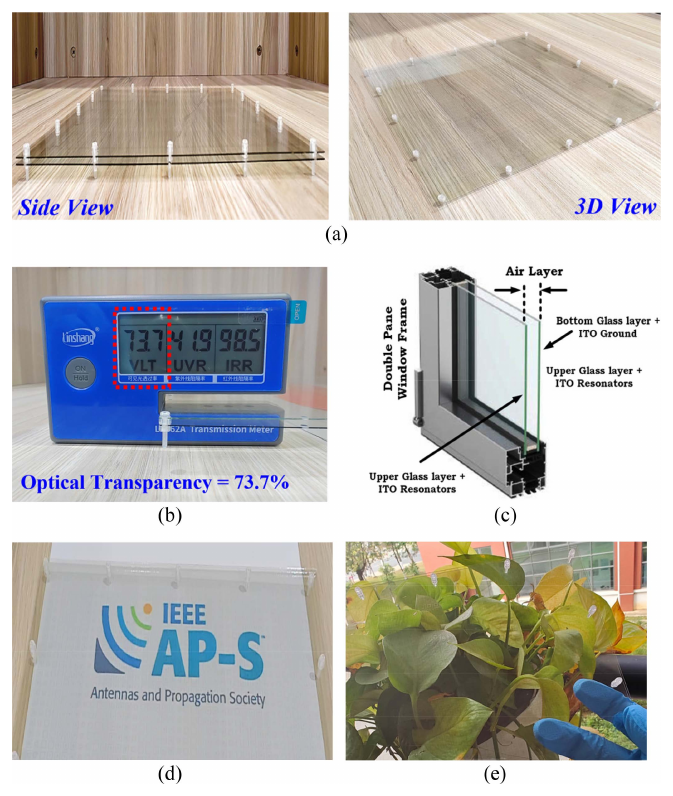
\includegraphics[width=0.6\textwidth]{Images/ch3_alnuaimi_fig9.png}
    \caption[Fabricated optically transparent EMS]{Fabricated transparent EMS: (a) side and 3D views, (b) measured optical transparency of 73.7\%, (c) integration into a double-pane window, (d), (e) visibility of objects behind the EMS (reprinted from~\cite{AlNuaimi2026}, \textcopyright~2025 IEEE).}
    \label{fig:ch3-prototype}
\end{figure}

\subsection{Limitations of the Approach}
\begin{itemize}
    \item ITO is a lossy conductor. The unit-cell loss stays below 4~dB at 26 and 28~GHz, but it grows with $R_{\mathrm{sheet}}$ (ohmic loss). Lowering it requires a lower $R_{\mathrm{sheet}}$, i.e., a thicker film, and 2.5~$\Omega$/sq was the lowest value available from the manufacturer~\cite{AlNuaimi2026}.
    \item The EMS is passive, with a single fixed reflection direction ($37^\circ$) and a small aperture ($200 \times 200$~mm).
    \item It was tested only in an anechoic chamber with horn antennas, not on a real building with a 5G BS.
\end{itemize}

\subsection{Results and Evaluation}
Table~\ref{tab:ch3-summary} summarizes the design and the measured performance. In both simulation and measurement, the reflected beam stays at $\theta_r = 37^\circ \pm 3^\circ$ from 24 to 30~GHz, i.e., over both n258 and n257. Anomalous reflection is strong and the specular lobe is much weaker~\cite{AlNuaimi2026}. Holding the angle within $\pm 3^\circ$ over a 6~GHz band is the main strength of the work, because one panel serves both 5G bands. The authors credit the unit-cell design for this: two cell types plus an air gap keep the phase stable across frequency.

The measured optical transparency is 73.7\% over 380--760~nm, and printed text and leaves behind the panel remain clearly visible (Fig.~\ref{fig:ch3-prototype}(d) and (e)). Measured and simulated reflections agree well. The authors attribute the small differences to three causes: misalignment of the setup, a change of the glass permittivity at mmWave frequencies, and a measured $R_{\mathrm{sheet}}$ of 2.25--2.29~$\Omega$/sq (mean 2.27~$\Omega$/sq) instead of the nominal 2.5~$\Omega$/sq~\cite{AlNuaimi2026}. The paper does not report the absolute reflected power or a link budget, so the coverage gain in a real gap cannot yet be quantified.

\begin{table}[!htbp]
    \centering
    \caption[Design parameters and performance of the transparent EMS]{Design parameters and performance of the optically transparent EMS~\cite{AlNuaimi2026}.}
    \label{tab:ch3-summary}
    \small
    \begin{tabularx}{\textwidth}{l >{\raggedright\arraybackslash}X}
        \toprule
        Item & Value \\
        \midrule
        Target bands & n258 (24.25--27.5~GHz) and n257 (26.5--29.5~GHz) \\
        Conductor and substrate & ITO, 2.5~$\Omega$/sq (650~nm), on two soda-lime glass layers with a 1~mm air gap \\
        Unit cells & two octagonal ITO cells, $0^\circ$--$360^\circ$ phase, period $0.42\lambda$ (26~GHz) and $0.45\lambda$ (28~GHz) \\
        Unit-cell loss & below 4~dB at 26 and 28~GHz \\
        Array & $40 \times 40$ cells, $200 \times 200 \times 2.1$~mm \\
        Design angles & $\theta_i = 15^\circ$ (BS at 10~m), $\theta_r = 37^\circ$ \\
        Reflection angle (simulated and measured) & $37^\circ \pm 3^\circ$ over 24--30~GHz \\
        Optical transparency (measured) & 73.7\% over 380--760~nm \\
        Measured $R_{\mathrm{sheet}}$ & 2.25--2.29~$\Omega$/sq (mean 2.27~$\Omega$/sq) \\
        \bottomrule
    \end{tabularx}
\end{table}

\subsection{Open Issues and Future Directions}
Lower-loss transparent conductors would recover part of the cell loss of up to 4~dB. Field trials on real windows with a commercial BS are still needed, as are larger or tiled panels that capture more power and a quantitative coverage study of the target gap. Finally, the reflection direction is fixed at design time; transparent skins that can be reconfigured to follow users remain an open topic.
